\documentclass[12pt,a4paper]{article}
\usepackage[utf8]{inputenc} % For UTF-8 encoding
\usepackage{amsmath, amssymb} % For mathematical symbols
\usepackage{graphicx} % For including images
\usepackage{hyperref} % For clickable links
\usepackage{geometry} % For page margins
\usepackage{booktabs} % For nice tables
\usepackage{lipsum} % For dummy text
\usepackage{longtable}
\usepackage{algorithm}
\usepackage{algorithmic}
\usepackage[style=apa, sorting=nyt, backend=biber]{biblatex} % Use biber as the backend
\addbibresource{references.bib}

\setlength{\parindent}{0em}
% Page layout
\geometry{margin=1in}

% Hyperlink setup
\hypersetup{
    colorlinks=true,
    linkcolor=blue,
    filecolor=magenta,
    urlcolor=cyan,
    pdftitle={LaTeX Template},
    pdfpagemode=FullScreen,
}

% ######################## Title  Page ####################################
\title{Recurrent Deep Learning Models and its applications}
\author{Ngai Ho Wang}

\date{\today}

\begin{document}

\maketitle
% ######################## Title  Page ####################################

% ######################## table of content ###############################
\tableofcontents % Generate a table of contents                        
% ######################## table of content ###############################

\newpage
% ######################## Introduction ####################################
\section{Introduction}

With the rise of the Generative Artificial Intelligence, the development of AI has already made remarkable strides in processing sequential data. In understanding and producing sequential data. It has applications ranging from Natural Language Processing (NLP) to music composition to video generation. Especially NLP, has emerged as a pivotal field in artificial intelligence, enable machines to understand, interpret and generate in human readable format. Some famous Artificial Intellience assistence for example, Siri, Alexa and Bixby have shown the possibility. Everyone can communicate with those machines, which make the reasonable response back to user.\\[1ex]
Recurrent Neural Networks (RNNs) have been a foundational architecture in this domain, Unlike the traditional Artificial Neural Network, RNNs do not treat each input independently, RNNs handle each input by considering the information from previous inputs. Conceptually this architecture able to retain the information. Thus, this architecture is suitable for handling sequential data. Unfortunately, early RNNs had limitation in training of networks over long sequence. vanishing and exploding gradient problems significantly affect the training process of RNN \parencite{bengio1994learning}. Eliminating many practical applications of RNNs. After that, \parencite{hochreiter1997lstm} introduced Long Short-Term Memory (LSTM) networks and are responsible for the breakthrough in how to solve these challenges. Specificized gating mechanisms were introduced in LSTMs to regulate the flow of the information, minimize the vanishing gradient problem and learn the long-term dependencies. This advanced made RNNs much more performant on tasks like a language modeling, machine translation and speech recognition tasks.\\[1ex]
Further improvements were achieved with Gated Recurrent Units (GRUs) by \parencite{cho2014properties} which diminished the LSTM architecture's complexity, but still provided the same performance. GRUs performed comparably but used fewer parameters, making it computationally and more tractably trainable.\\[1ex]
Since the craze of AI has been revived by generative AI, natural language processing to time series prediction and speech recognition have once again aroused people's interest in RNN. This report aims to:
\begin{itemize}
    \item Explore the theoretical foundations of recurrent deep learning models.
    \item Investigate their diverse applications in solving sequential data tasks.
    \item Analyze their performance, strengths, and inherent limitations.
\end{itemize}
% ######################## Introduction ####################################
\newpage
% ######################## Background and Literature Review #########################
% Background and Literature Review 
\section{Background and Literature Review}
% Evolution of Deep Learning and Recurrent Neural Networks 
\subsection{Evolution of Deep Learning and Recurrent Neural Networks}
In the past few decades, thank to the rapidly development of technology, the computing resource has a incredible increase. Thus, substantially deep learning architecture have improved, from simple architectures, which only able to capture simple information from data to sophisticated models that are able to learn complex, abstract representations. This was before the early neural networks like perceptrons and multilayer perceptrons (MLPs) laid the footwork of neural computation that first came in the picture, but were burdened by the lack of ability to model sequential dependencies. This however imposed a limit on the feed forward paradigm, which prompted the development of recurrent neural networks (RNNs) that extend the old stalactite of feed forward paradigm with cyclic connections. Through these connection, RNNs are capable to keep a hidden state that represents information over time steps thereby effectively capture temporal dynamics. RNNs have been a decisive step in the evolution of deep learning, as they are able to do tasks that require memory of previous events, including problems of natural language processing and time series modeling. Despite that, early RNNs models suffered from serious problems for example,  vanishing gradients and exploding gradients, which prevented these RNN models from learning long ranged dependencies. This stimulated the building of more refined architectures intended to side step these obstacles.

\newpage

% Literature Review
\subsection{Literature Review}
% Backpropagation Through Time
\subsubsection{Backpropagation Through Time}
BPTT is one of the most important algorithms used for training RNNs. Dating back to the original effort to expand the typical backpropagation algorithm, BPTT has been formulated to handle the difficulties of temporal sequences that are inherent in sequential data \parencite{werbos1990bptt}. This algorithm allows RNNs in learning sequence dependent data by unfold the network over time steps and then updating weights matrix through the gradient of loss function with respect to the variable \parencite{rumelhart1986backpropagation}.
\\[2ex]
\textbf{Conceptual Framework of BPTT}
\\[1ex]
BPTT works based on the technique of treating an RNN as a deep feedforward network for across multiple time steps. In the forward pass, the RNN, like other artificial neuronal network, applies operation over the data input in sequence, bringing changes in its own state variables at every time step, depending on the input and the previous state of its general working state or hidden state. This sequential processing produces outputs and stores the internal states of the network in any period \parencite{werbos1990bptt}.

This unfolds the RNN to construct a traditional Feedforward Neural Network where we can apply backpropagation through time. Below is the conceptual idea of BPTT in RNN.
\begin{figure}[h!]
    \centering
    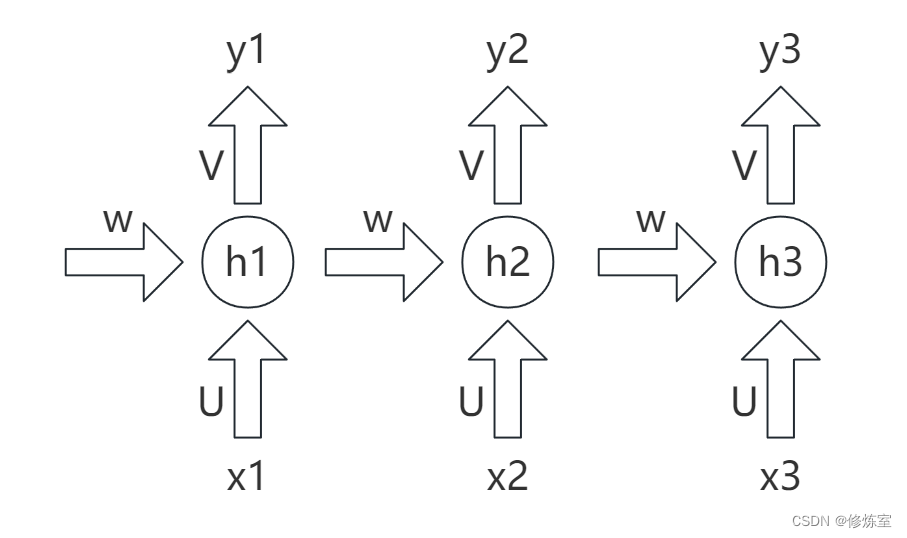
\includegraphics[width=1\textwidth]{../Pic/pic1.png} % Replace "example-image" with your image file
    \caption{Unfolded RNN}
\end{figure}

\newpage
\begin{longtable}{|c|c|c|}
    \hline
    \textbf{Notation} & \textbf{Meaning} & \textbf{Dimension}\\
    \hline
    $U$          & Weight matrix for input to hidden state       & $input\ size\times hidden\ unites$\\
    $W$          & Weight matrix for hidden to hidden state      & $hidden\ units\times hidden\ unites$\\
    $V$          & Weight matrix for hidden state to output state& $hidden\ units\times number\ of\ class$\\
    $x_t$        & Input vector at time t                        & $input\ size\times 1$\\
    $h_t$        & Hidden state output at time t                 & $hidden\ units\times 1$\\
    $b_h$        & Bias term for hidden state                    & $hidden\ units\times 1$\\
    $b_y$        & Bias term for output state                    & $number\ of\ class\times 1$\\
    $\hat{o}_y$  & Output at time t                              & $number\ of\ class\times 1$\\
    $\hat{y}_t$  & Output at time t                              & $hidden\ units\times 1$\\
    $\mathcal{L}$& Loss at time t                                & $scalar$\\
    \hline
    \caption{Unfolded RNN}
\end{longtable}
% Forward pass
\noindent \textbf{Forward Pass}
\\[1ex]
During the forward pass, the RNN processes the input sequence sequentially, computing hidden states and output at each timestep:
\begin{equation}
    h_t = f(U^Tx_{t}+W^Th_{t-1}+b_h)
\end{equation}
\begin{equation}
    \hat{y}_t = f(V^Th_t+b_y)
\end{equation}
\newline  % Computing the loss function
\noindent \textbf{Computing the loss function}
\\[1ex]
Assuming the loss is computed only at the final timestep t:
\begin{equation}
    \mathcal{L}_t = L(y_t, \hat{y}_t)
\end{equation}
In order to do backpropagation through time to tune the parameters in RNN, we need to calculate the partial derivative of loss function $\mathcal{L}$ with respect to the differently parameters.\\
\newline  % Backward pass using the chain rule
\noindent \textbf{Backward pass using the chain rule}
\\[1ex]
Using the chain rule for computing the gradient.\\
Partial derivative of loss function $\mathcal{L}$ with respect to $W$ (hidden to hidden state) at time 2. 
\begin{equation}
    \dfrac{\partial\mathcal{L}_2}{\partial W} = \dfrac{\partial\mathcal{L}_2}{\partial y_2} \cdot \dfrac{\partial y_2}{\partial h_2} \cdot \dfrac{\partial h_2}{\partial h_1} \cdot \dfrac{\partial h_1}{\partial W}
\end{equation}
By mathematic induction 
\begin{equation}
    \dfrac{\partial\mathcal{L}_t}{\partial W} = \dfrac{\partial\mathcal{L}_t}{\partial y_t} \cdot \dfrac{\partial y_t}{\partial h_t} \cdot (\sum_{i=1}^{t} \dfrac{\partial h_t}{\partial h_i} \cdot \dfrac{\partial h_i}{\partial W})
\end{equation}
Where 
\begin{equation}
    \dfrac{\partial h_t}{\partial h_i} = \prod_{j=i+1}^{t} \dfrac{\partial h_j}{\partial h_{j-1}}
\end{equation}

Partial derivative of loss function $\mathcal{L}$ with respect to $U$ (input to hidden state) at time 2.\\
\begin{equation}
    \dfrac{\partial\mathcal{L}_2}{\partial U} = \dfrac{\partial\mathcal{L}_2}{\partial y_2} \cdot \dfrac{\partial y_2}{\partial h_2} \cdot \dfrac{\partial h_2}{\partial h_1} \cdot \dfrac{\partial h_1}{\partial U}
\end{equation}
By mathematic induction 
\begin{equation}
    \dfrac{\partial\mathcal{L}_t}{\partial U} = \dfrac{\partial\mathcal{L}_t}{\partial y_t} \cdot \dfrac{\partial y_t}{\partial h_t} \cdot (\sum_{i=1}^{t} \dfrac{\partial h_t}{\partial h_i} \cdot \dfrac{\partial h_i}{\partial U})
\end{equation}
Where 
\begin{equation}
    \dfrac{\partial h_t}{\partial h_i} = \prod_{j=i+1}^{t} \dfrac{\partial h_j}{\partial h_{j-1}}
\end{equation}

Partial derivative of loss function $\mathcal{L}$ with respect to $V$ (hidden to output state) at time 2.\\
\begin{equation}
    \dfrac{\partial\mathcal{L}_2}{\partial V} = \dfrac{\partial\mathcal{L}_2}{\partial y_2} \cdot \dfrac{\partial y_2}{\partial h_2} \cdot \dfrac{\partial h_2}{\partial h_1} \cdot \dfrac{\partial h_1}{\partial V}
\end{equation}
By mathematic induction 
\begin{equation}
    \dfrac{\partial\mathcal{L}_t}{\partial V} = \dfrac{\partial\mathcal{L}_t}{\partial y_t} \cdot \dfrac{\partial y_t}{\partial h_t} \cdot (\sum_{i=1}^{t} \dfrac{\partial h_t}{\partial h_i} \cdot \dfrac{\partial h_i}{\partial V})
\end{equation}
Where 
\begin{equation}
    \dfrac{\partial h_t}{\partial h_i} = \prod_{j=i+1}^{t} \dfrac{\partial h_j}{\partial h_{j-1}}
\end{equation}

Partial derivative of loss function $\mathcal{L}$ with respect to $b_h$ (bias term in hidden state) at time 2.\\
\begin{equation}
    \dfrac{\partial\mathcal{L}_2}{\partial b_b} = \dfrac{\partial\mathcal{L}_2}{\partial y_2} \cdot \dfrac{\partial y_2}{\partial h_2} \cdot \dfrac{\partial h_2}{\partial h_1} \cdot \dfrac{\partial h_1}{\partial b_h}
\end{equation}
By mathematic induction 
\begin{equation}
    \dfrac{\partial\mathcal{L}_t}{\partial b_h} = \dfrac{\partial\mathcal{L}_t}{\partial y_t} \cdot \dfrac{\partial y_t}{\partial h_t} \cdot (\sum_{i=1}^{t} \dfrac{\partial h_t}{\partial h_i} \cdot \dfrac{\partial h_i}{\partial b_h})
\end{equation}
Where 
\begin{equation}
    \dfrac{\partial h_t}{\partial h_i} = \prod_{j=i+1}^{t} \dfrac{\partial h_j}{\partial h_{j-1}}
\end{equation}

Partial derivative of loss function $\mathcal{L}$ with respect to $b_y$ (bias term in output state) at time 2.
\begin{equation}
    \dfrac{\partial\mathcal{L}_2}{\partial b_y} = \dfrac{\partial\mathcal{L}_2}{\partial y_2} \cdot \dfrac{\partial y_2}{\partial h_2} \cdot \dfrac{\partial h_2}{\partial h_1} \cdot \dfrac{\partial h_1}{\partial b_y}
\end{equation}
By mathematic induction 
\begin{equation}
    \dfrac{\partial\mathcal{L}_t}{\partial b_y} = \dfrac{\partial\mathcal{L}_t}{\partial y_t} \cdot \dfrac{\partial y_t}{\partial h_t} \cdot (\sum_{i=1}^{t} \dfrac{\partial h_t}{\partial h_i} \cdot \dfrac{\partial h_i}{\partial b_y})
\end{equation}
Where 
\begin{equation}
    \dfrac{\partial h_t}{\partial h_i} = \prod_{j=i+1}^{t} \dfrac{\partial h_j}{\partial h_{j-1}}
\end{equation}

\textbf{parameters updates}
\begin{equation}
    W \leftarrow W - \alpha\dfrac{\partial\mathcal{L}}{\partial W}
\end{equation}
\begin{equation}
    U \leftarrow U - \alpha\dfrac{\partial\mathcal{L}}{\partial U}
\end{equation}
\begin{equation}
    V \leftarrow V - \alpha\dfrac{\partial\mathcal{L}}{\partial V}
\end{equation}
\begin{equation}
    b_h \leftarrow b_h - \alpha\dfrac{\partial\mathcal{L}}{\partial b_h}
\end{equation}
\begin{equation}
    b_y \leftarrow b_y - \alpha\dfrac{\partial\mathcal{L}}{\partial b_y}
\end{equation}

\textbf{Pseudocode of BPTT} \parencite{wikipedia2023bptt}
\begin{algorithm}[H]
    \caption{Backpropagation Through Time (BPTT)}
    \begin{algorithmic}[1]
    \STATE \textbf{Input:} 
    \STATE \hspace{1em} Sequence of input data $\{x_1, x_2, \dots, x_T\}$
    \STATE \hspace{1em} Sequence of target outputs $\{y_1, y_2, \dots, y_T\}$
    \STATE \hspace{1em} Learning rate $\eta$
    \STATE \hspace{1em} Number of time steps to unroll $N$
    \STATE \textbf{Initialize:} Model parameters $\theta$, hidden state $h_0 = 0$
    
    \STATE \textbf{Forward Pass:}
    \FOR{$t = 1$ to $T$}
        \STATE Compute hidden state: $h_t = f(h_{t-1}, x_t; \theta)$
        \STATE Compute output: $\hat{y}_t = g(h_t; \theta)$
        \STATE Compute loss for time step $t$: $L_t = \mathcal{L}(\hat{y}_t, y_t)$
    \ENDFOR
    
    \STATE \textbf{Backward Pass (BPTT):}
    \STATE Set total loss: $L = \sum_{t=1}^{T} L_t$
    \FOR{$t = T$ down to $1$}
        \STATE Compute gradient of loss with respect to output: $\frac{\partial L_t}{\partial \hat{y}_t}$
        \STATE Backpropagate through output layer to obtain: $\frac{\partial L_t}{\partial h_t}$
        \STATE Accumulate gradients for parameters: $\frac{\partial L}{\partial \theta}$
        \FOR{$k = 1$ to $N$}
            \STATE Backpropagate through time for $N$ steps:
            \STATE Compute gradient contribution from step $t-k$: $\frac{\partial L_t}{\partial h_{t-k}}$
        \ENDFOR
    \ENDFOR
    
    \STATE \textbf{Update Parameters:}
    \STATE $\theta = \theta - \eta \cdot \frac{\partial L}{\partial \theta}$
    
    \STATE \textbf{Output:} Updated parameters $\theta$
    \end{algorithmic}
\end{algorithm}

\newpage
% Actication function
\subsubsection{Activation Function}
Activation functions, particularly the sigmoid function, are fundamental components of recurrent neural networks (RNNs). They transform input data into output data. A key property of these functions is their differentiability. Differentiability is crucial for the backpropagation through time (BPTT) algorithm, enabling the application of the chain rule during training. \\[1ex]
% Sigmoid Activation Function 
\textbf{Sigmoid activation function}
\\[1ex]
The main role of the sigmoid activation function is to normalize candidate values and convert the cell state to a hidden state when performing cell state updates. It limits the output between [0,1] because it has a smooth gradient, which is important for discovering long-range dependencies.\\[1ex]
\begin{equation}
    Sigmoid(x) = \frac{ 1 }{ 1+e^{-x} }
\end{equation}
\begin{equation}
    Sigmoid'(x) = Sigmoid(x)(1-Sigmoid(x))
\end{equation}
Below is the sigmoid function and its derivative.
\begin{figure}[!htb]
    \centering
    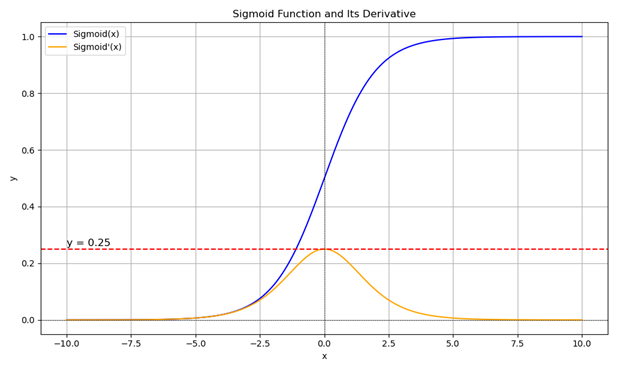
\includegraphics[width=1\textwidth]{../Pic/sigmoid.png} % Replace "example-image" with your image file
    % \caption{An example image.}
    \label{fig:sigmoid}
\end{figure}
\newline
$Domain(Sigmoid(x))=\mathbb{R},\hspace{1em} Codomain(Sigmoid(x))=(0,1)$\\
$Domain(Sigmoid'(x))=\mathbb{R},\hspace{1em} Codomain(Sigmoid'(x))=[0,0.5]$

% Hyperbolic tangent activation function
\newpage
\textbf{Hyperbolic tangent activation function}
\\[1ex]
The main role of the hyperbolic tangent (tanh) activation function is to normalize candidate values and convert the cell state to a hidden state when performing cell state updates. It limits the output between [-1,1] because it has a stable gradient, which is important for discovering long-range dependencies.
\newline
\begin{equation}
    tanh(x) = \frac{ e^{x} - e^{-x} }{e^{x} + e^{-x}}
\end{equation}
\begin{equation}
    tanh'(x) = 1 - tanh^{2}(x)
\end{equation}
Below is the Hyperbolic tangent activation function and its derivative.\\
\begin{figure}[!htb]
    \centering
    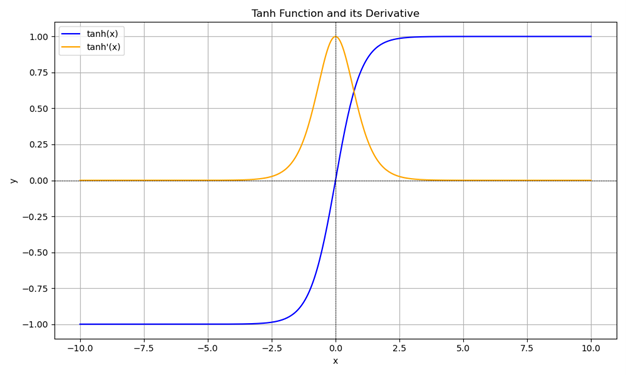
\includegraphics[width=1\textwidth]{../Pic/tanh.png} % Replace "example-image" with your image file
    % \caption{An example image.}
    \label{fig:tanh}
\end{figure}
\newline
$Domain(tanh(x))=\mathbb{R},\hspace{1em} Codomain(tanh(x))=[-1,1]$\\
$Domain(tanh'(x))=\mathbb{R},\hspace{1em} Codomain(tanh'(x))=[0,1]$

% Gradient vanishing and gradient exploring
\newpage
\subsubsection{Gradient vanishing and gradient exploring}
When training the RNN, BPTT was used to update the weight matrix. As the number of time steps increase, the problem of gradient instability of often encountered, and this problem is gradient vanishing and gradient explored \parencite{bengio1994learning}. 
\\[2ex]
% Vanishing Gradients
\textbf{Vanishing Gradients}
\\[1ex]
Generally, sigmoid activation function is used commonly in RNNs, has a maximum derivative of 0.25. When doing BPTT in long time steps, this multiplication results in exponentially diminishing gradients as the sequence length increases. Consequently, the shallow neural receive very small gradient updates, making it difficult to adjust the parameters effectively. This leads to the model struggling to learn long time dependencies. 
\\[1ex]
% Exploding Gradients
\textbf{Exploding Gradients}
\\[1ex]
When we are doing the feedforward and get super large value computed by loss function. Then when updating the parameters. The updates to the weights will also be large. Resulting in higher loss and larger gradients in the next iterations. This will lead to exploding gradients.
\\[1ex]
We have introduce the backpropagation through time. This is the method to update the parameters in RNNs. When calculating, for example, the partial derivative of loss function with respect to W. Assume the time $t$ go to infinity large. We will get this term. $ \prod_{j=i+1}^{t} \dfrac{\partial h_j}{\partial h_{j-1}} $, and it will lead to exponential problem. if $ \dfrac{\partial h_j}{\partial h_{j-1}} > 1 $. Then the product of all term will increase exponentially, then exploding gradients occur. On the contrary, if $\dfrac{\partial h_j}{\partial h_{j-1}} < 1$. Then the result will decrease exponentially, then vanishing gradients occur.
\begin{figure}[!htb]
    \centering
    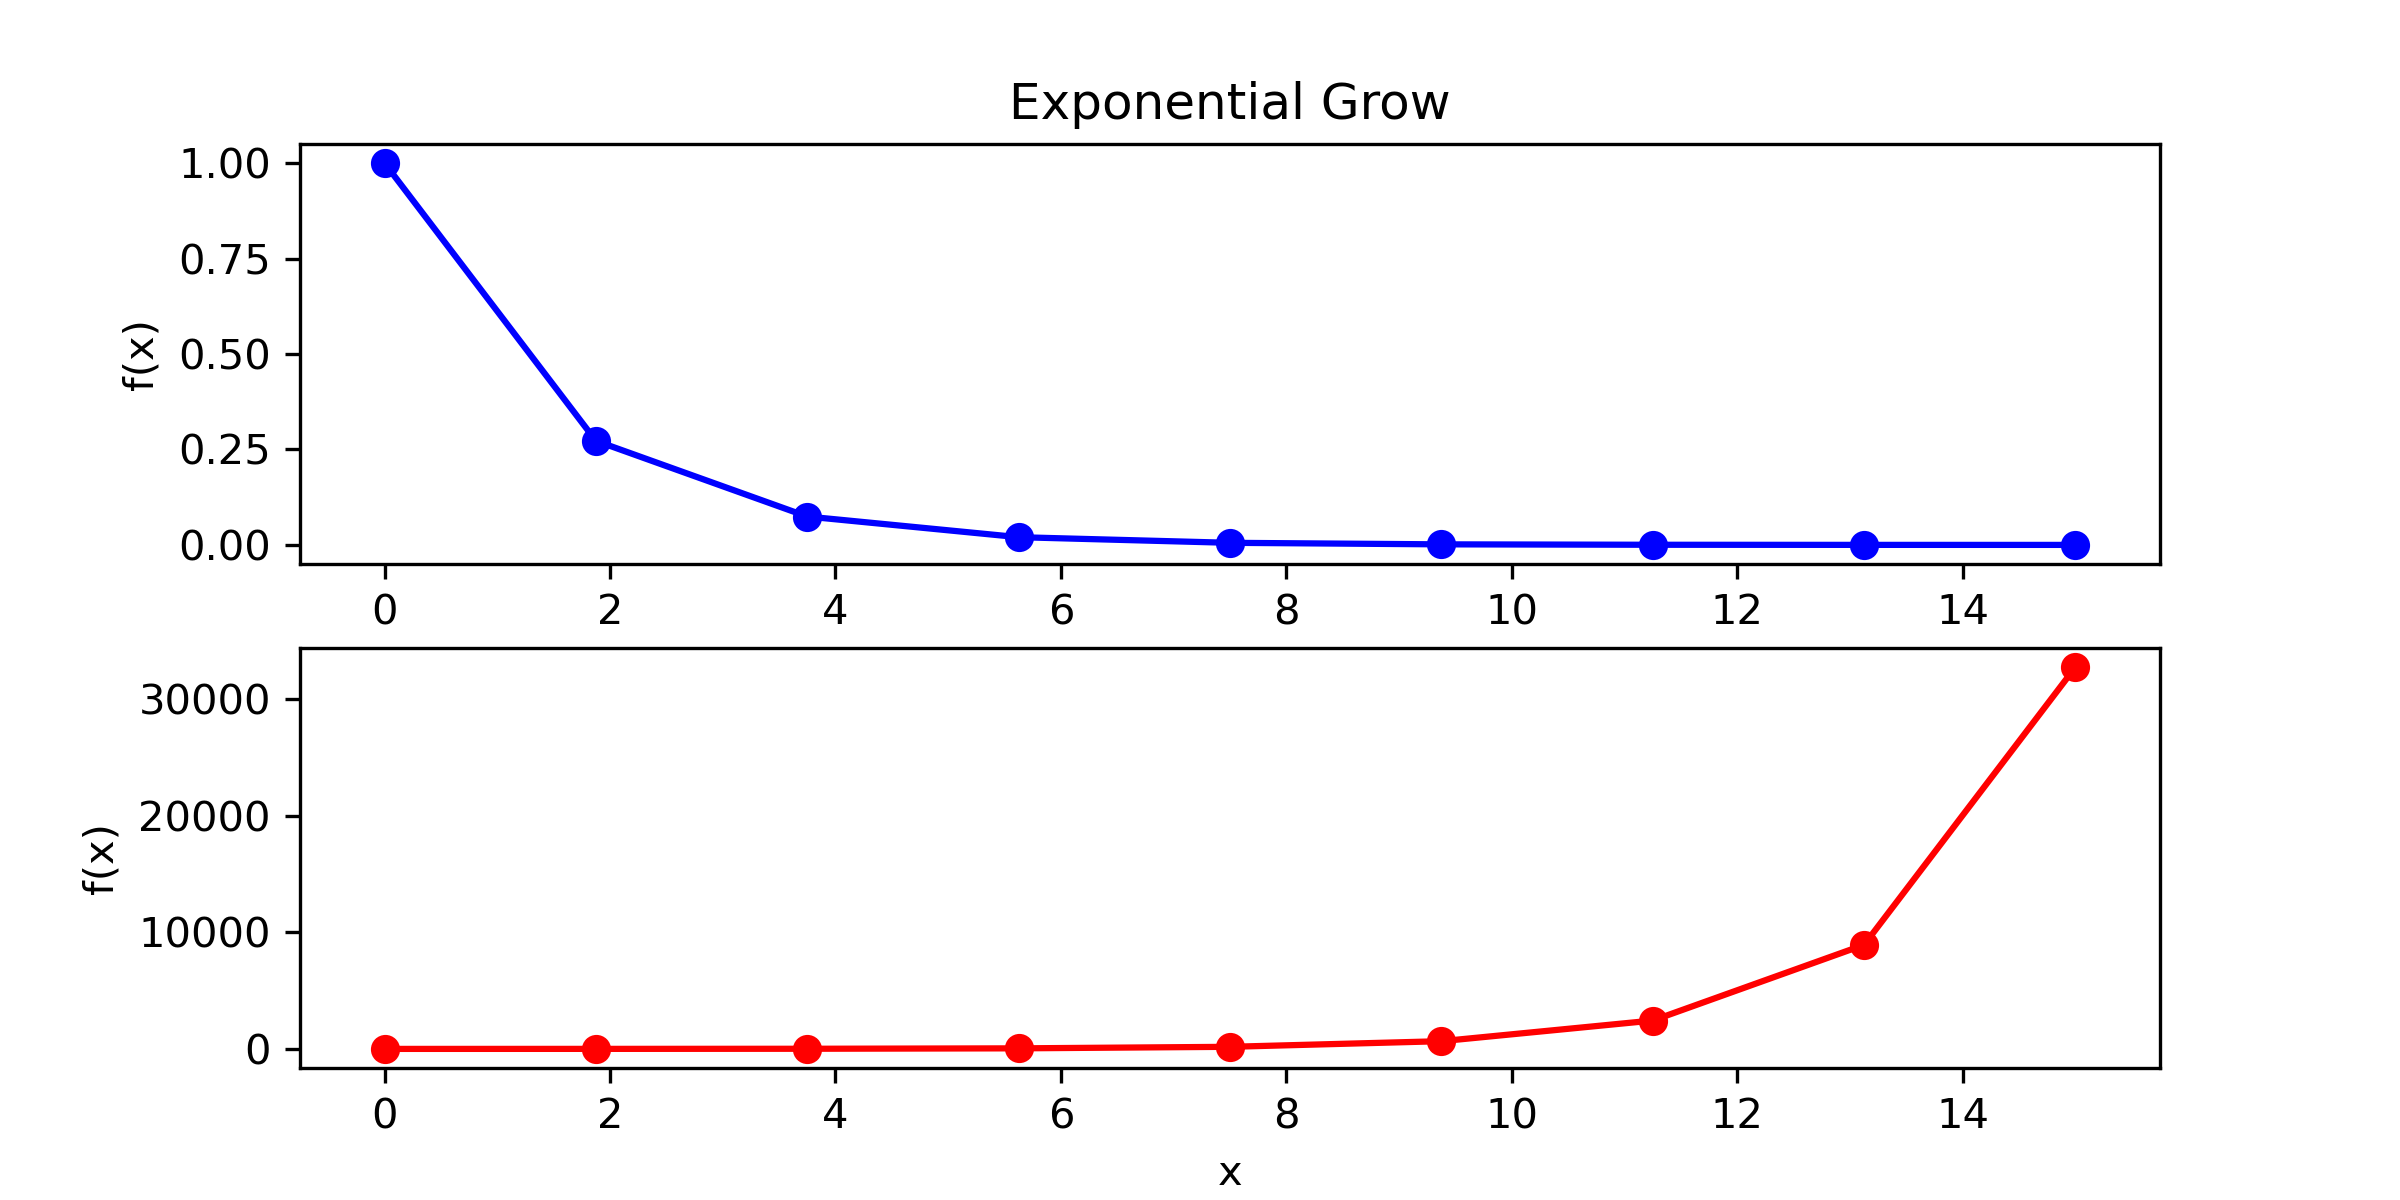
\includegraphics[width=1\textwidth]{../Pic/exponential_growth.png} % Replace "example-image" with your image file
\end{figure}


\newpage
% Long short-term memory (LSTM)
\subsubsection{Long short-term memory (LSTM)}
Long short-term memory proposed by \parencite{hochreiter1997lstm}. LSTM is designed for handling long time step problems. The architecture of LSTM can prevent vanishing gradient and exploring gradient. The main difference between LSTM and RNN is the number of gates. LSTM introduced input, forget and output gates. This allows LSTM to manage the flow of information more effectively, retaining important information over longer sequences.
\\[2ex]
Architecture
\\[1ex]
LSTMs introduce a memory cell that can maintain information over long time steps the cell is controlled by three gates, input gate, output gate, and forget gate. Each cell of LSTMs inside has 3 sigmoid and 1 tanh layer. Below graph unfolds the LSTM hence we can analyze different gates.
\begin{figure}[!htb]
    \centering
    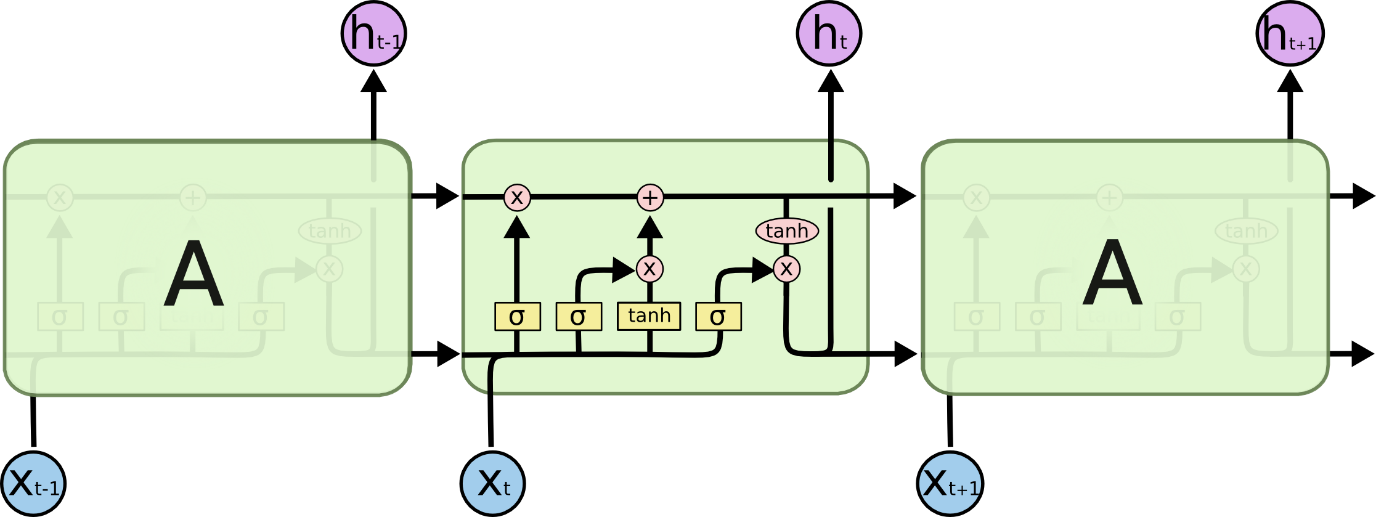
\includegraphics[width=1\textwidth]{../Pic/lstm1.png} % Replace "example-image" with your image file
\end{figure}
\begin{figure}[!htb]
    \centering
    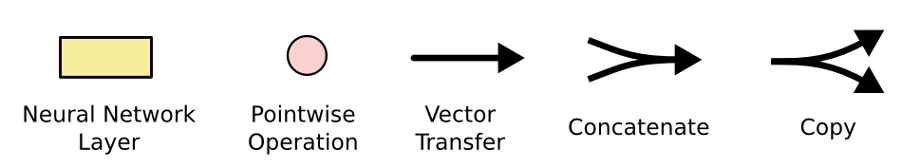
\includegraphics[width=1\textwidth]{../Pic/lstm2.png} % Replace "example-image" with your image file
\end{figure}
\\
% Forget gate
Forget gate:
\\[1ex]
The forget gate is a component of the LSTM, designed to manage the flow of information within the cell state. The function of forget gate is to determine which information should be retained in memory cell \parencite{hochreiter1997lstm}.
\begin{equation}
    f_t = \sigma( W_f \cdot [ h_{t-1} , x_t ] + b_f ) 
\end{equation}
% Input gate
Input gate: 
\\[1ex]
The input gate controls how much new information from the current time step is allowed to enter the cell \parencite{hochreiter1997lstm}. For the $\widetilde{C}_t$, the purpose is to suggest updates for the cell state. 
\begin{equation}
    i_t = \sigma( W_i \cdot [ h_{t-1} , x_t ] + b_c ) 
\end{equation}
\begin{equation}
    \widetilde{C}_t = tanh( W_c \cdot [ h_{t-1} , x_t ] + b_c )
\end{equation}
% Cell state update
Cell State Update:
\\[1ex]
The forget gate will drop the meaningless information and add some potential information.
\begin{equation}
    C_t = f_t * C_{t-1} + i_t * \widetilde{C_t}
\end{equation}
% Output gate
Output gate:
\\[1ex]
The output gate is able to control how much or what information from the cell state should be passed to the next layer or used in predictions. 
\begin{equation}
    o_t = \sigma( W_o \cdot [ h_{t-1} , x_t ] + b_o )
\end{equation}
% Hidden state update
Hidden State Update:
\\[1ex]
The hidden state is influenced by output value and current cell state. 
\begin{equation}
    h_t = o_t * tanh(C_t)
\end{equation}
\\[1ex]
n = number of features in the input vector $x_t$.\\
m = number of units in LSTM.\\
\begin{longtable}{|c|c|c|}
    \hline
    \textbf{Notation} & \textbf{Meaning} & \textbf{Dimension}\\
    \hline
    $x_t$               & Input vector at time t                        & $n \times 1$\\
    $h_t$               & Hidden state output at time t                 & $m \times 1$\\
    $C_t$               & Cell state at time t                          & $m \times 1$\\
    $f_t$               & Forget gate output at time t                  & $m \times 1$\\
    $i_t$               & Input gate output at time t                   & $m \times 1$\\
    $o_t$               & Output gate output at time t                  & $m \times 1$\\
    $\widetilde{C_t}$   & Candidate memory cell at time t               & $m \times 1$\\
    $W_f$               & Weight matrix for the forget gate             & $m \times (m+n)$\\
    $W_i$               & Weight matrix for the input gate              & $m \times (m+n)$\\
    $W_C$               & Weight matrix for the candidate memory cell   & $m \times (m+n)$\\
    $W_o$               & Weight matrix for the output gate             & $m \times (m+n)$\\
    $b_f$               & Bias vector for the forget gate               & $m \times 1$\\
    $b_i$               & Bias vector for the input gate                & $m \times 1$\\
    $b_C$               & Bias vector for the candidate memory cell     & $m \times 1$\\
    $b_o$               & Bias vector for the output gate               & $m \times 1$\\
    \hline
    \caption{Unfolded RNN}
\end{longtable}

Number of parameters:\\
\begin{enumerate}
    % 1. Weights matrix for the input
    \item Weights matrix for the input
    \begin{itemize}
        \item Forget gate: $n \times m$
        \item Input gate: $n \times m$
        \item Cell gate: $n \times m$
        \item Output gate: $n \times m$
    \end{itemize}

    % 2. Weight matrix for the hidden state
    \item Weight matrix for the hidden state
    \begin{itemize}
        \item Hidden state for forget gate: $m \times m$
        \item Hidden state for input gate: $m \times m$
        \item Hidden state for cell gate: $m \times m$
        \item Hidden state for output gate: $m \times m$
    \end{itemize}

    % 3. Bias term
    \item Bias term
    \begin{itemize}
        \item Bias for forget gate: $1 \times m$
        \item Bias for input gate: $1 \times m$
        \item Bias for cell gate: $1 \times m$
        \item Bias for output gate: $1 \times m$
    \end{itemize}
\end{enumerate}
Total parameters: $4 \times ( n + m + 1 ) \times m$


\newpage
% Gated Recurrent Unit (GRU)
\subsubsection{Gated Recurrent Unit (GRU)}
The gated recurrent unit (GRU) was proposed by \parencite{cho2014properties} to make each recurrent unit to adaptively capture dependencies of different time scales. The GRU has 2 gates, update gate and reset gate. 
\begin{figure}[!htb]
    \centering
    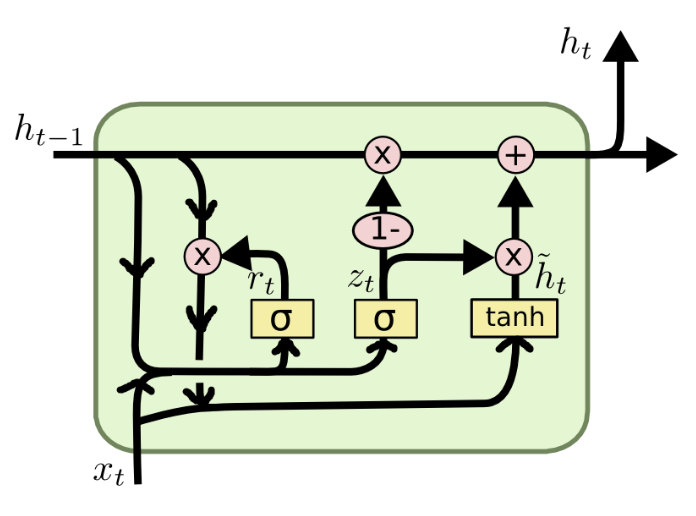
\includegraphics[width=0.65\textwidth]{../Pic/gru.png} % Replace "example-image" with your image file
\end{figure}
Update gate:
\\[1ex]
The update gate determines how much of the past information should be retained in the current hidden state. 
\begin{equation}
    z_t = \sigma(W_z \cdot [ h_{t-1} , x_t ] + b_z )
\end{equation}
% Reset gate
Reset gate:
\\[1ex]
The reset gate is similar with the update gate, but the candidate hidden state is influenced by the reset gate. 
\begin{equation}
    r_t = \sigma( W_r \cdot [ h_{t-1} , x_t ] + b_r )
\end{equation}
Candidate hidden state:
\\[1ex]
The candidate hidden state combined with previous hidden state and current input to form the potential new information that can be added to the current hidden state.
\begin{equation}
    \widetilde{h_t} = tanh ( W_h \cdot [ r_t * h_{t-1} , x_t ] + b_h )
\end{equation}
Final hidden state
\\[1ex]
The final hidden state of the GRU at time t is a linear interpolation between the previous final hidden state and the candidate hidden state. 
\begin{equation}
    h_t = ( 1 - z_t ) * h_{t-1} + z_t * \widetilde{ h_t }
\end{equation}

\begin{longtable}{|c|c|c|}
    \hline
    \textbf{Notation} & \textbf{Meaning} & \textbf{Dimension}\\
    \hline
    $x_t$               & Input vector at time t                        & $n \times 1$\\
    $h_t$               & Hidden state output at time t                 & $m \times 1$\\
    $r_t$               & Reset gate output at time t                   & $m \times 1$\\
    $z_t$               & Update gate output at time t                  & $m \times 1$\\
    $W_z$               & Weight matrix for the update gate             & $m \times (m+n)$\\
    $W_r$               & Weight matrix for the candidate memory cell   & $m \times (m+n)$\\
    $W_h$               & Weight matrix for the output gate             & $m \times (m+n)$\\
    $b_z$               & Bias vector for the input gate                & $m \times 1$\\
    $b_r$               & Bias vector for the candidate memory cell     & $m \times 1$\\
    $b_h$               & Bias vector for the output gate               & $m \times 1$\\
    \hline
\end{longtable}

Number of parameters:\\
\begin{enumerate}
    % 1. Weights matrix for the input
    \item Weights matrix for the input
    \begin{itemize}
        \item Update gate: $n \times m$
        \item Reset gate: $n \times m$
        \item Candidate hidden state: $n \times m$
    \end{itemize}

    % 2. Weight matrix for the hidden state
    \item Weight matrix for the hidden state
    \begin{itemize}
        \item Hidden state for update gate: $m \times m$
        \item Hidden state for reset gate: $m \times m$
        \item Hidden state candidate hidden state: $m \times m$
    \end{itemize}

    % 3. Bias term
    \item Bias term
    \begin{itemize}
        \item Bias for update: $1 \times m$
        \item Bias for reset: $1 \times m$
        \item Bias for candidate hidden state: $1 \times m$
    \end{itemize}
\end{enumerate}
Total parameters: $3 \times ( n + m + 1 ) \times m$
\newpage


% Deep recurrent neural networks (DRNNs)
\subsubsection{Deep recurrent neural networks (DRNNs)}
Deep architecture networks with multiple layers that can hierarchically learn complex representations \parencite{bengio2009learning}. By extending of this concept, stacking recurrent layers to form Deep Recurrent Neural Networks aligns with this principle. A number of research papers have been prove that the performance of DRNNs is out-performance then conventional RNNs. \parencite{le2010deep, delalleau2011shallow, pascanu2013on}
\\[1ex]
The architecture of DRNNs are similar with conventional RNNs. We simply stack the recurrent layers vertically. For the first layer, this layer receives the input and combines it with its previous hidden state $h_{t-1}$ (Equation 38). The second layer receive the hidden state of the first layer and treat as the input of the layer 2 (Equation 39). We can extend this concept to $L$ layers (Equation 40).
\begin{figure}[!htb]
    \centering
    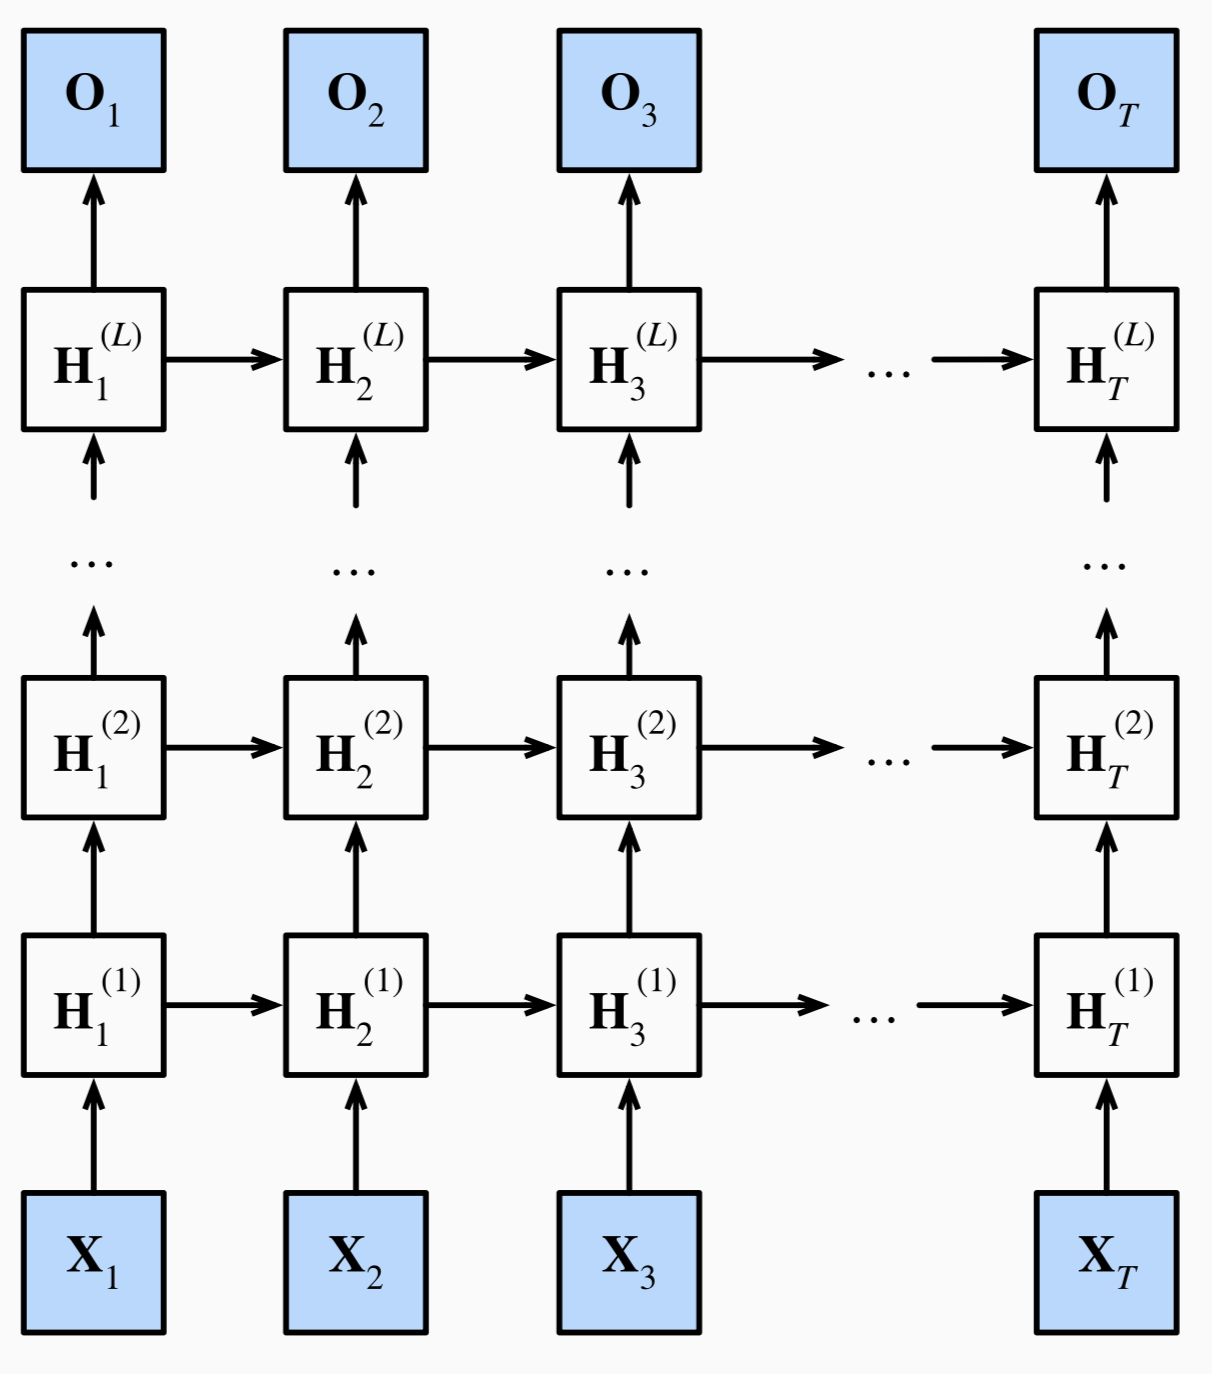
\includegraphics[width=0.5\textwidth]{../Pic/drnn.png} % Replace "example-image" with your image file
\end{figure}
\\[1ex]
\begin{equation}
    h^{(1)}_t = f(W^{(1)}_{xh} x_{t} + W^{(1)}_{hh} h^{(1)}_{t-1} + b^{(1)}_h)
\end{equation}
\begin{equation}
    h^{(2)}_t = f(W^{(2)}_{xh} h^{(1)}_{t} + W^{(2)}_{hh} h^{(2)}_{t-1} + b^{(2)}_h)
\end{equation}
\begin{equation}
    h^{(L)}_t = f(W^{(L)}_{xh} h^{(L-1)}_{t} + W^{(L)}_{hh} h^{(L)}_{t-1} + b^{(L)}_h)
\end{equation}
\begin{equation}
    o_t = W_{hy}h^{(L)}_{t} + b_y
\end{equation}
\begin{equation}
    y_t = g(o_t)
\end{equation}
Where $x_t$ is the input at time $t$. $h^{(l)}_{t}$ is the hidden state for the $l$ layer at time t. $W^{(l)}_{xh}, W^{(l)}_{hh}$ are the weight matrices for the input to hidden and hidden to hidden connections in layer $l$, respectively. $W_{hy}$ is weight matrix for the output layer. $b^{(l)}_h$ is the bias vector for the $l$ layer (except output layer), $b_y$ is the bias vector for output layer. $g(\cdot)$ and $f(\cdot)$ are an activation function. 

\newpage
\subsubsection{Hidden Markov Model}
Before reviewing Hidden Markov Model (HMM), it is essential to understand what Markov models is, or Markov chains. Markov chains are fundamental models in probability theory and statistic, and it is a stochastic process describing a sequence of possible events in which the probability of each event depends only on the state attained in the previous event. This property known as the Markov property \parencite{roberts2004general, rabiner1986anintroduction}. In rigorous terms. Let the state space be defined as:
\begin{equation}
    S = \{ s_1, s_2, \dots, s_N \}.
\end{equation}
\begin{equation}
    P(s_{t+1} \mid s_t, s_{t-1}, s_{t-2}, \cdots, s_{1}) = P(s_{t+1} \mid s_t)
\end{equation}
The state transition probability is denoted by:
\begin{equation}
    P_{ij} = P(s_{t+1} = s_j \mid s_t = s_i).
\end{equation}

Given an initial state \( s_1 \) with probability \( P(s_1) \), the joint probability of a state sequence \( \{s_1, s_2, \dots, s_T\} \) can be written as:
\begin{equation}
    P(s_1, s_2, \dots, s_T) = P(s_1) \cdot P(s_2 \mid s_1) \cdot P(s_3 \mid s_2) \cdots P(s_T \mid s_{T-1})
\end{equation}
We can simplfy the joint probability of a state sequence as equestion 47.
\begin{equation}
    P(s_1, s_2, \dots, s_T) = P(s_1) \prod_{t=1}^{T-1} P(s_{t+1} \mid s_{t})
\end{equation}
Then it is essential to discuss marginal probability in a Markov model because it provides critical information about the likelihood of being in particular state $s_j$ at a specific time $t$. The marginal probability of being in state $s_j$ at time $t$ defined as:
\begin{equation}
    \pi_t(s_j) = P(s_t=s_j)
\end{equation}
It is the probability of the system being in state $s_j$ at time t, irrespective of how the system transitioned to $s_j$. We can obtainde by summing over all possible transition probability $P_{ij}$ where $s_i$ belong in state space. 
\begin{equation}
    \pi_{t+1}(s_j) = \sum_{s_i \in S} \pi_t(s_i) \cdot P_{ij}
\end{equation}
If Markov chain is irreducible and aperiodic, the stationary distribution defined as below:
\begin{equation}
    \pi_j = \sum_{i=1}^{n} \pi_i P_{ij}
\end{equation}

\newpage

% Hidden markov model 
\textbf{Hidden markov model}
\\[1ex]
Hidden Markov Model (HMMs) is a statistical model that extends the Markov chains by introducting a layer of latent (unobservable) variables. And connecting them to observable outputs (emission probability). In contrast to standard Markov chains, hidden states are never be observed directly. Instead, we observe a sequence of data (observations) that are probabilitically generated by these hidden state. This structure has proven useful for applications in speech recognition, biological sequence analysis, and signal processing \parencite{rabiner1989atutorial}. Lets the hidden states be denoted by $X_t$, where $X_t$ is the hidden state at time $t$. The hidden state space is defined as:
\begin{equation}
    \mathcal{X} = \{s_1, s_2, \cdots, s_n\}
\end{equation}
where $\mathcal{X}$ is finite set of size $n$, and each $s_i \in \mathcal{X}$ represents a specific possible hidden state. Then for the observable space represents the possible outcomes (observations) that are generated by the hidden state, we have discuss previously. Let the observations at time $t$ be denoted by $Y_t$. The observable space is defined as:
\begin{equation}
    \mathcal{Y} = \{o_1, o_2, \cdots, o_m\}
\end{equation}
where $\mathcal{Y}$ is finite set of size $m$, and each $o_i \in \mathcal{Y}$ represents a specific possible observation. 
\\[1ex]
Then for the transition probability matrix ($P$), the probability of transitioning between hidden states denoted as:
\begin{equation}
    P_{n \times n} = 
    \left[ {\begin{array}{cccc}
        p_{11} & p_{12} & \cdots & p_{1n}\\
        p_{21} & p_{22} & \cdots & p_{2n}\\
        \vdots & \vdots & \ddots & \vdots\\
        p_{n1} & p_{n2} & \cdots & p_{nn}\\
    \end{array} } \right]
\end{equation}
\begin{equation}
    p_{ij} = P(X_{t+1} = s_j \mid X_t = s_i) 
\end{equation}
where $s_j, s_i \in \mathcal{X}$.
\\[1ex]
For emission probability matrix ($B$), the probabilities of generating an observation given a hidden state.
\begin{equation}
    B_{n \times n} = 
    \left[ {\begin{array}{cccc}
        b_{11} & b_{12} & \cdots & b_{1m}\\
        b_{21} & b_{22} & \cdots & b_{2m}\\
        \vdots & \vdots & \ddots & \vdots\\
        b_{m1} & b_{m2} & \cdots & b_{mm}\\
    \end{array} } \right]
\end{equation}
\begin{equation}
    b_{ik} = P(Y_{t} = o_k \mid X_t = s_i) 
\end{equation}
where $s_i \in \mathcal{X}, o_k \in \mathcal{Y}$.
\\[1ex]
And the goal of hidden markov model is the maximize the joint probability $P(X, Y)$ given the initial probability $P(X_1)$.
\begin{equation}
    P(X, Y) = P(X_1) \cdot \prod_{t=1}^{T-1}P(X_{t+1}=s_j \mid X_{t}=s_i) \cdot \prod_{t=1}^{T} P(Y_t=o_k \mid X_t=s_i)
\end{equation}

For the NLP tasks, there may have some unobservable data, for example the implicit sentiment, user intent, emotional state. \parencite{rabiner1993fundamentals} proposes the hidden Markov model (HMM), the assumption is the existence of the latent process follows a Markov chain from which observations X are generated. In other word, there would exists an unobserved state sequence $Z = \{z_1, z_2 \cdots , z_T\}$ in observed sequence $X = \{x_1, x_2, \cdots, x_T\}$ \parencite{sengupta2023hybrid}. Where the hidden states, $z_t$ belonging to state-space $Q = \{q_1, q_2, \cdots, q_M \}$ follow a Markov chain goverened by: 
\begin{itemize}
    \item A state-transition probability matrix $A = [a_{ij}] \in \mathbb{R}^{M \times M}$ where $a_{ij} = p(z_{t+1} = q_j | z_t = q_i)$ 
\end{itemize}
\begin{itemize}
    \item Initial state matrix $\pi = [\pi_i] \in \mathbb{R}_{1 \times M}$ with $\pi_i = p(z_1 = q_i)$
\end{itemize}
Furthermore, for the hidden state $z_t$, correspoinding to the observe data $x_t$ is release by emission process $B = [b_j(x)]$ where $b_j(x) = p(x|z=q_i)$. We can assume $b_j(x)$ is follows the Gaussian mixture model (GMM).
\begin{equation}
    p(x_t|z=q_j) = \sum_{l=1}^{k}c_{jl}\mathcal{N}(x_t|\mu_{jl}, \Sigma_{jl})
\end{equation}
where $\sum_{l=1}^{k}c_{jl} = 1$, $\forall j = \{1,\cdots, M\}$, k is the number of Gaussian mixture components and $\mathcal{N}(x_t|\mu_{jl}, \Sigma_{jl})$ denotes a Gaussian probability density with mean $\mu_{jl}$ and covariance $\Sigma_{jl}$ for state $j$ and mixture component $l$. The number of hidden states ($M$) and mixture component ($k$) are the two hyperparameters of the model which have to be provided apriori.
\\[1ex]
Therefore, the joint probability probability density function of the observation $X$ can be expressed as:
\begin{equation}
    p(X) = p(z_1) \prod_{t=1}^{T-1} p(z_{t+1}|z_{t}) \prod_{t=1}^{T} p(x_t|z_t)
\end{equation}
The optimal parameters $[A, B, \pi]$, which maximize the likelihood of the observation sequence $X$ (Equation 39), are determined using the Baum-Welch algorithm, an expectation-maximization method \parencite{rabiner1993fundamentals}. Additionally, the probability of the system in a specific hidden state $z_t$ corresponding to the observation $x_t$ is calculated using the Viterbi algorithm.

\newpage

% Word representation 
\subsubsection{Word representation}
In RNN, the due to the architecture, the model can only handle vector, it is important that convert the word into machine readable format. By translating words into vectors, these representations capture semantic meanings, relationships and contexts. \parencite{mikolov2013efficient} proposed 2 model architectures for leaning distributed representations of words.
\\[1ex]
\textbf{Continuous Bag of Words model}
CBOW operates by taking context words around a target word, it is flexible to adjust the window size which mean that we can control how many words around our target word. Hence aggregating their embeddings and passing to hidden layer to produce a probability distribution. Capture the semantic meanings and the relationship more effectively. 
\begin{equation}
    Q = N \times D + D \times log_2(V)
\end{equation}
\\[1ex]
\textbf{Continuous Skip gram model}
\\[1ex]
The continuous skip gram model operates in opposite direction compare with CBOW. The model takes the surrounding word to predict the target word. In other word, treat the current word as an input to a log-linear classifier with continuous projection layer, and predict the probability distribution of surrounding words.
\begin{equation}
    Q = C \times (D + D \times log_2(V))
\end{equation}
\begin{figure}[!htb]
    \centering
    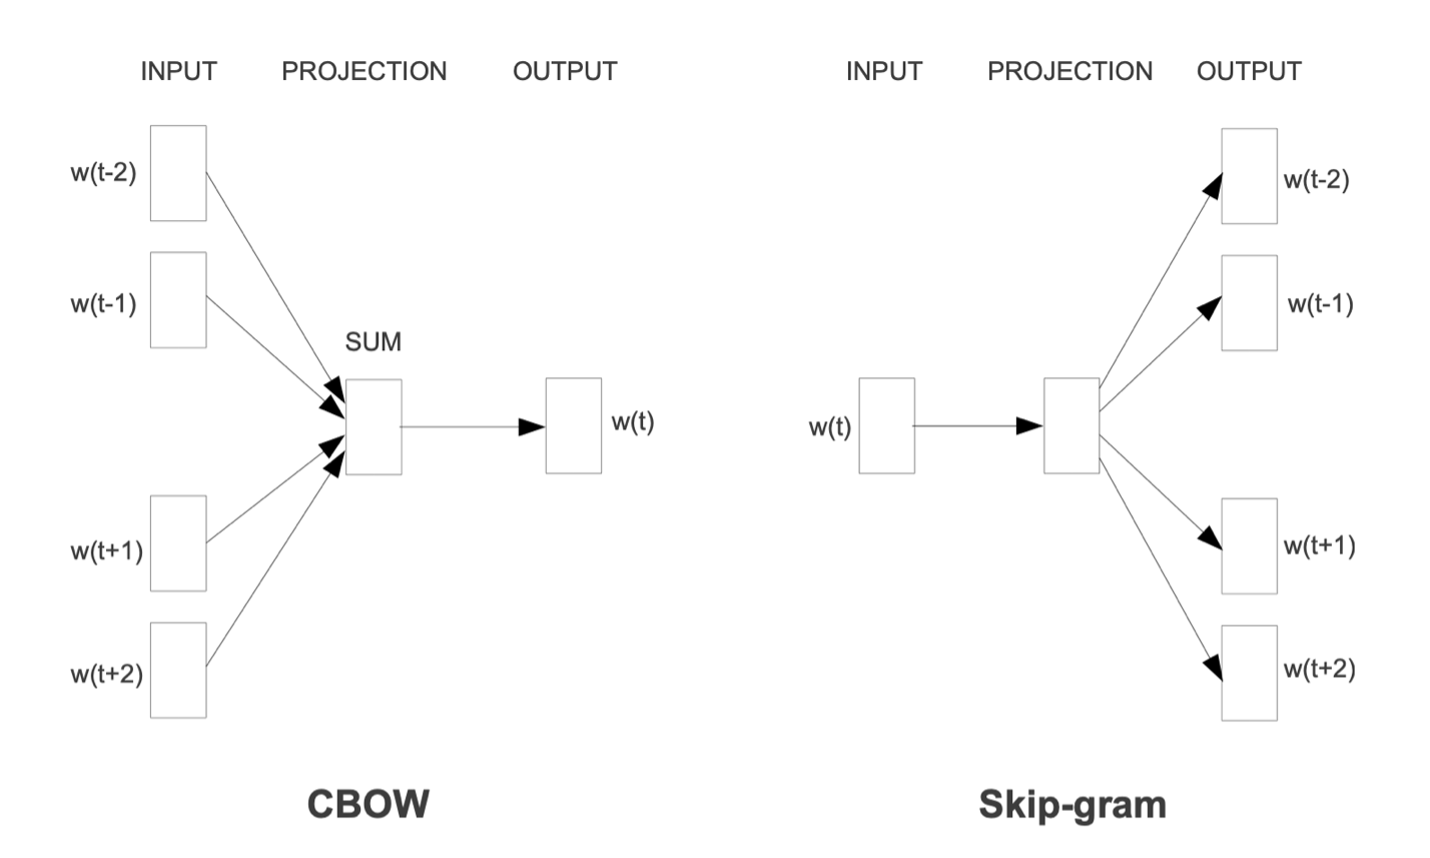
\includegraphics[width=1\textwidth]{../Pic/word_representation.png} % Replace "example-image" with your image file
\end{figure}

\newpage


% ######################## Background and Literature Review #########################

% ######################## Reference ######################################
\printbibliography
% ######################## Reference ######################################

\end{document}